\documentclass[a4paper]{article}
\usepackage[]{float}
\usepackage[utf8]{inputenc}
\usepackage[T1]{fontenc}
\usepackage{textcomp}
\usepackage[dutch]{babel}
\usepackage{amsmath, amssymb}
\usepackage{tikz}
\usepackage{amsmath}
\usepackage{physics}
\usepackage{pgfplots}
\usepackage{caption}
\usepackage{gensymb}
\usepackage[margin=2cm]{geometry}
\usepackage{import}
\usepackage{xifthen}
\pdfminorversion=7
\usepackage{pdfpages}
\usepackage{transparent}
\newcommand{\incfig}[1]{%
	\def\svgwidth{\columnwidth}
	\import{./figures/}{#1.pdf_tex}
}

\pdfsuppresswarningpagegroup=1
\newcommand{\hb}{\hbar}
\begin{document}
\begin{center}
	\begin{huge}
		PHYS 202: Homework 11
	\end{huge}\\ 
	\
	\\
	\begin{Large}
		Ahmed Saad Sabit
	\end{Large}
\end{center}	
\section*{Problem 01} 
\[
F_z = \mu_z \alpha
\] 
\[
t = \frac{L}{v}
\] 
\[
d = \frac{1}{2} (\frac{F_z}{m}) t^2 = \frac{1}{2} 
\left(
\frac{\mu_z \alpha}{m}
\right)
\left(\frac{L}{v}\right)^2 \implies  \alpha = 
\frac{2 m v^2 d }{\mu_z L^2}  =
\boxed{
0.386
}
\] 

\section*{Problem 02}
\subsection*{(a)} 
\[
p \sim \frac{\hb}{r} = 1.05 \times 10^{-16} \text{ kg m/s}
\] 
\[
v = p  / m = 1.2 \times 10^{14} \text{ m/s} \gg 3.0 \times 10^{8} \text{ m/s} = c
\] 
This speed is extreme and un-relativistic thus unreal. 

\subsection*{(b)} 
\[
E \sim pc = \frac{\hb c}{r} = 2 \times 10^{5} \text{ MeV}
\] 
But rest energy of electron is $0.511 \text{ MeV}$. The classically flawed energy ratio is
\[
\frac{E}{0.511 } = 4 \times  10 ^{5} 
\] 
This is unrealistically high proportion of energy. 






\section*{Problem 03}
\subsection*{(a)} 
Comparing wiht $n^2 \hb ^2 \pi ^2 / 2 m L ^2$ we see that 
\[
n_1 ^2 + n_2 ^2 = 5
\] 
The only valid pairs that solve this above equation are 
\[
n_1 = 1, n_2 = 2 
\] 
or
\[
n_2 = 2, n_1 = 1
\] 
So the occupied states are $n = 1,2$.

\subsection*{(b)} 
\[
\psi_S (x_1, x_2) = 
\frac{1}{\sqrt{2} } 
\left(
\psi_1(x_1) \psi_2(x_2) + \psi_2(x_1) \psi_1(x_2)
\right) \implies \sqrt{2}  \psi_1(x_1) \psi_2(x_1)
\] 
Wave functions are given for $n$ state by 
\[
\sqrt{\frac{2}{L}} \sin\left(\frac{n \pi x}{L}\right)
\] 
Plotting in desmos for $L = 1$ for $n = 1,2$ 
\begin{figure}[H]
	\centering
	
\includegraphics[width=0.8\textwidth]{./pics/1.png}
	
\includegraphics[width=0.8\textwidth]{./pics/3.png}
	\caption{Wave Function and Probability Plot}
	\label{fig:-pics-1-png}
\end{figure}


\subsection*{(c)} 

\[
\psi_A (x_1, x_2) = 
\frac{1}{\sqrt{2} } 
\left(
\psi_1(x_1) \psi_2(x_2) - \psi_2(x_1) \psi_1(x_2)
\right) \underbrace{\implies}_{x_1 = x_2} \quad 0
\] 

\begin{figure}[H]
	\centering
	
\includegraphics[width=0.8\textwidth]{./pics/2.png}
	\caption{Wave Function (and so as probability)}
	\label{fig:-pics-2-png}
\end{figure}

\subsection*{(d)} 
Symmetric wave function plot with $L-x$ 
\begin{figure}[H]
	\centering
	
\includegraphics[width=0.8\textwidth]{./pics/4.png}
	\caption{./pics/4.png}
	\label{fig:-pics-4-png}
\end{figure}


Asymmetric Wave Function and Probability for $L-x$ 
\begin{figure}[H]
	\centering
	
\includegraphics[width=0.8\textwidth]{./pics/5.png}
	\caption{./pics/5.png}
	\label{fig:-pics-5-png}
\end{figure}





\section*{Problem 04} 
\subsection*{Spin Half} 
Fermions are spin half. So each energy state can hold two of them for the two eigenvalues of the spins. For this 
\[
E_1 \implies 2 \] \[ 
E_2 \implies 2 \] \[
E_3 \implies 1
\]
Total energy 
\[
E = \frac{\pi^2 \hb^2}{2 m L^2} (2(1^2) + 2(2^2 ) + 3^2) = \boxed{
19 \frac{\pi ^2 \hb ^2}{2 m L ^2}
}
\] 

\subsection*{Spin one} 
Spin 1 are bosons so they all can take ground state for minimum energy
\[
\boxed{
E = 5 \frac{\pi^2 \hb^2}{2 m L^2}
}\] 



\subsection*{Spin 3/2}
Again fermions, but this time the eigenvalues of spin are 
\[
\frac{3}{2} , \frac{1}{2}, - \frac{1}{2}, - \frac{3}{2}
\] 
So 4 of the lowest energy states can be filled up with 4 eigenvalues of the spin and the rest remaining is the $n = 2$ state hence we have $4 + (2)^2 = 8$ 
\[\boxed{
E = 8 \frac{\pi^2 \hb^2}{2 m L^2}
} \] 




\section*{Problem 05}
\subsection*{(a)}
Swap for spatial part in state $I$ 
\[
	I = \psi_n(x_1) \uparrow  \psi_{n'} (x_2) \downarrow 
	- 
	\psi_{n'}(x_1) \downarrow \psi_n (x_2) \uparrow 
	\implies 
	\psi_{n'}(x_1) \uparrow  \psi_{n} (x_2) \downarrow 
	- 
	\psi_{n}(x_1) \downarrow \psi_{n'} (x_2) \uparrow = - I I 
\]
Spatial state swap for $I$ gives us $- I I $. This also implies that swapping the states of $I I $ will give us $- I$. 

Now we cannot call this either symmetric or antisymmetric because the swap is not positive of negative of it self - rather we have a totally different state (as we saw swapping $I$ gives $ - I I $).

To be able to call $I$ antisymmetric, we need the swap to give us $- I $ state, not $- I I$.

\[
\boxed{
\text{Neither.}
}
\] 


\subsection*{(b)}
Swap the spin part of states,
\[
	I = \psi_n(x_1) \uparrow  \psi_{n'} (x_2) \downarrow 
	- 
	\psi_{n'}(x_1) \downarrow \psi_n (x_2) \uparrow 
	\implies 
	\psi_n(x_1) \downarrow  \psi_{n'} (x_2) \uparrow 
	- 
	\psi_{n'}(x_1) \uparrow \psi_n (x_2) \downarrow  = I I 
\]
Spin swaps for $I$ gave us $I I $ states, hence it's obvious that swapping spin states for $I I $ would give us $I$ state. Hence again, because the swapped states are neither $+$ or $-$ of themselves, we are left with the exchange symmetry being neither symmetric or antisymmetric.

\[
\boxed{
\text{Neither.}
}
\]


\subsection*{(c)}
	\[ 
		I + I I = 
		\left( 
			\psi_n(x_1) \uparrow  \psi_{n'} (x_2) \downarrow 
	- 
	\psi_{n'}(x_1) \downarrow \psi_n (x_2) \uparrow  \right) 
	+ \left(\psi_n(x_1) \downarrow  \psi_{n'} (x_2) \uparrow 
	- 
	\psi_{n'}(x_1) \uparrow \psi_n (x_2) \downarrow  \right) 
\]
Notationally making a change, 
		\[ 
			\left( 
			\psi_n(x_1)   \psi_{n'} (x_2) \uparrow \downarrow 
	- 
	\psi_{n'}(x_1) \psi_n (x_2) \downarrow \uparrow  \right) 
	+ \left(\psi_n(x_1) \psi_{n'} (x_2) \downarrow \uparrow 
	- 
	\psi_{n'}(x_1) \psi_n (x_2) \uparrow \downarrow  \right)  
\] 
		\[ 
			\left( 
			\psi_n(x_1)   \psi_{n'} (x_2) \right) (\uparrow \downarrow  + \downarrow \uparrow)
	- 
	\psi_{n'}(x_1) \psi_n (x_2) (\downarrow \uparrow  
	+ \uparrow \downarrow  )
\] 
		\[\boxed{
			\left[ 
			\psi_n(x_1)   \psi_{n'} (x_2) - 
			\psi_{n'}(x_1) \psi_n (x_2) \right] (\downarrow \uparrow  
		+ \uparrow \downarrow  )
	}
\] 


\subsection*{(d)} 
Spatial swap 
\[
			\left[ 
			\psi_n(x_1)   \psi_{n'} (x_2) - 
			\psi_{n'}(x_1) \psi_n (x_2) \right] (\downarrow \uparrow  
		+ \uparrow \downarrow  )
			\implies 
			\left[ 
				\psi_{n'}(x_1)   \psi_{n} (x_2) - 
			\psi_{n}(x_1) \psi_{n'} (x_2) \right] (\downarrow \uparrow  
		+ \uparrow \downarrow  )
\] 
\[
\implies 
			- \left[ 
			\psi_n(x_1)   \psi_{n'} (x_2) - 
			\psi_{n'}(x_1) \psi_n (x_2) \right] (\downarrow \uparrow  
		+ \uparrow \downarrow  )
\]
Quite obviously
\[
\boxed{
\text{Spatially Antisymmetric}
}\] 

Spin Swap
			\[ 
				\left[ 
			\psi_n(x_1)   \psi_{n'} (x_2) - 
			\psi_{n'}(x_1) \psi_n (x_2) \right] (\downarrow \uparrow  
		+ \uparrow \downarrow  ) 
				\implies 
				\left[ 
			\psi_n(x_1)   \psi_{n'} (x_2) - 
			\psi_{n'}(x_1) \psi_n (x_2) \right]
			\underbrace{(  
			\uparrow \downarrow + \downarrow \uparrow) }_{\text{look here bro}}
	\]
			\[ 
			\implies 	\left[ 
			\psi_n(x_1)   \psi_{n'} (x_2) - 
			\psi_{n'}(x_1) \psi_n (x_2) \right] (\downarrow \uparrow  
		+ \uparrow \downarrow  )  \]
We got the same thing 
\[
\boxed{
\text{Spininically Symmetric}
}
\] 


\subsection*{(e)} 
Spin exchange symmetry implies unchanged states. Hence if we change both spatial and spin part, then only spatial acts to make the whole state negative hence keeping it anti-symmetric.
\[
\boxed{
\text{Still Anti-symmetric.}
}
\] 

\subsection*{(f)}
Repulsion requires the particles to be kept farther apart. Now in state $I$ and $I I $ we have such case that $x_1 = x_2$ can still give non-zero probability of existing, whereas \textit{sum} case give zero probability for $x_1 = x_2$. Hence the \textit{sum} case more likely because repulsion makes it less likely for the particles to be at the same position (or close).  




\section*{Problem 06}
\begin{align*}
\psi_a &= \psi_{1,0,0}(\mathbf{r})\uparrow \\
\psi_b &= \psi_{1,0,0}(\mathbf{r})\downarrow \\
\psi_c &= \psi_{2,0,0}(\mathbf{r})\uparrow
\end{align*}

Slater Determinant is written 
\[
\Psi(\mathbf{r}_1, \mathbf{r}_2, \mathbf{r}_3) = \frac{1}{\sqrt{6}}
\begin{vmatrix}
\psi_{1,0,0}(\mathbf{r}_1)\uparrow & \psi_{1,0,0}(\mathbf{r}_2)\uparrow & \psi_{1,0,0}(\mathbf{r}_3)\uparrow \\
\psi_{1,0,0}(\mathbf{r}_1)\downarrow & \psi_{1,0,0}(\mathbf{r}_2)\downarrow & \psi_{1,0,0}(\mathbf{r}_3)\downarrow \\
\psi_{2,0,0}(\mathbf{r}_1)\uparrow & \psi_{2,0,0}(\mathbf{r}_2)\uparrow & \psi_{2,0,0}(\mathbf{r}_3)\uparrow \\
\end{vmatrix}
\]

The incredibly painful work of expanding this thing 
\[
\Psi = \frac{1}{\sqrt{6}} \Big(
\psi_{1,0,0}(\mathbf{r}_1)\uparrow \cdot \psi_{1,0,0}(\mathbf{r}_2)\downarrow \cdot \psi_{2,0,0}(\mathbf{r}_3)\uparrow
- \psi_{1,0,0}(\mathbf{r}_1)\uparrow \cdot \psi_{2,0,0}(\mathbf{r}_2)\uparrow \cdot \psi_{1,0,0}(\mathbf{r}_3)\downarrow
+ \psi_{1,0,0}(\mathbf{r}_2)\uparrow \cdot \psi_{2,0,0}(\mathbf{r}_3)\uparrow \cdot \psi_{1,0,0}(\mathbf{r}_1)\downarrow
\]
\[
- \psi_{1,0,0}(\mathbf{r}_2)\downarrow \cdot \psi_{1,0,0}(\mathbf{r}_3)\uparrow \cdot \psi_{2,0,0}(\mathbf{r}_1)\uparrow
+ \psi_{1,0,0}(\mathbf{r}_3)\uparrow \cdot \psi_{1,0,0}(\mathbf{r}_1)\downarrow \cdot \psi_{2,0,0}(\mathbf{r}_2)\uparrow
- \psi_{1,0,0}(\mathbf{r}_3)\uparrow \cdot \psi_{2,0,0}(\mathbf{r}_1)\uparrow \cdot \psi_{1,0,0}(\mathbf{r}_2)\downarrow
\Big)
\]
I counted 6 terms which is correct. 









\section*{Problem 07}

\subsection*{(a)} 
\[
B = \frac{\mu_0 I}{2 a} = \mu_0 \left(\frac{\mu_e}{\pi a^2}\right) \frac{1}{2 a} = 
\frac{\mu_0}{2a} \frac{e \hb}{2 m_e \pi a^2} = \frac{\mu_0 e \hb}{4 \pi m_e a^3}
\] 


\subsection*{(b)} 
It's a very basic fact in condensed matter physics that anti-aligned configuration is lower in energy. In a bar magnet idea too, north and north repel so it's more sustainable to have an opposite configuration hence anti-aligned is lower in energy (as it is stable). 

\subsection*{(c)} 
\[
\Delta E = 2 \mu_p B= 2 \left(5.6 \frac{e \hb}{2 m_p}\right) \left(\frac{\mu_0 e \hb}{4 \pi m_e a^3}\right) = 5.8 \times 10^{-6} \text{ eV}
\] 
\begin{figure}[H]
	\centering
	
\includegraphics[width=0.8\textwidth]{./pics/6.png}
	\caption{./pics/6.png}
	\label{fig:-pics-6-png}
\end{figure}

\subsection*{(d)} 
\[
E = \frac{hc}{\lambda} \implies \lambda = \frac{hc}{\Delta E}
\]
Calculator gives 
\[
E = 0.21 m = \boxed{
21 cm
}
\] 




\section*{Problem 08} 
\subsection*{(a)} 
Eigenvalues are (PHYS 311/312)
\[
\frac{3}{2}, \frac{1}{2}, - \frac{1}{2}, - \frac{3}{2}
\] 

\subsection*{(b)} 
\[
\cos\theta = \frac{S_z}{|\vec{S}|} = \frac{m_s \hbar}{\sqrt{s(s+1)}\hbar} = \frac{m_s}{\sqrt{s(s+1)}}
\]
\begin{align*}
m_s = \frac{3}{2} &\Rightarrow \cos\theta = \frac{3/2}{\sqrt{15}/2} = \frac{3}{\sqrt{15}} \Rightarrow \theta = \cos^{-1}\left( \frac{3}{\sqrt{15}} \right) \approx 35.26^\circ \\
m_s = \frac{1}{2} &\Rightarrow \cos\theta = \frac{1}{\sqrt{15}} \Rightarrow \theta = \cos^{-1}\left( \frac{1}{\sqrt{15}} \right) \approx 75.52^\circ \\
m_s = -\frac{1}{2} &\Rightarrow \cos\theta = -\frac{1}{\sqrt{15}} \Rightarrow \theta = \cos^{-1}\left( -\frac{1}{\sqrt{15}} \right) \approx 104.48^\circ \\
m_s = -\frac{3}{2} &\Rightarrow \cos\theta = -\frac{3}{\sqrt{15}} \Rightarrow \theta = \cos^{-1}\left( -\frac{3}{\sqrt{15}} \right) \approx 144.74^\circ
\end{align*}

\begin{center}
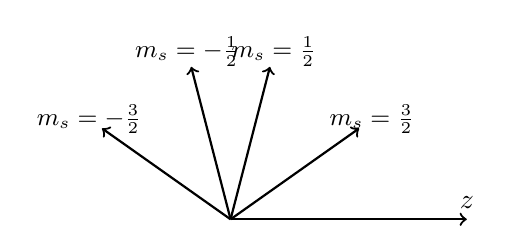
\begin{tikzpicture}[scale=2]

  % z-axis
  \draw[->, thick] (0,0) -- (1.5,0) node[above] {\( z \)};

  % Draw spin vectors at different angles
  \foreach \angle/\label in {
    35.26/{$m_s = \frac{3}{2}$},
    75.52/{$m_s = \frac{1}{2}$},
    104.48/{$m_s = -\frac{1}{2}$},
    144.74/{$m_s = -\frac{3}{2}$}
  } {
    \draw[->, thick] (0,0) -- ({cos(\angle)}, {sin(\angle)});
    \node at ({1.1*cos(\angle)}, {1.1*sin(\angle)}) {\small \label};
  }

\end{tikzpicture}

\vspace{1em}
\textbf{Spin-\( \frac{3}{2} \): Angles with the \( z \)-axis}
\end{center}


\subsection*{(c)}
Degeneracies are 4 fold for 4 possible eigenvalues of spin.
\end{document}
